\documentclass[11pt]{article}
\usepackage[margin=1in]{geometry}
\usepackage{amsmath,amssymb}
\usepackage{booktabs}
\usepackage{graphicx}
\usepackage{subcaption}
\usepackage{siunitx}

\title{Augmented Controller Explanation and Simulation Plots}
\date{}

\begin{document}
\maketitle

\section{Overview}
This report explains the augmented controller implemented in \texttt{augmented\_controller.py} and compares it against the baseline cascaded PID controller in a hover-with-wind test.

\section{Controller Structure}
The baseline controller outputs thrust and body moments through cascaded loops. The baseline outer position loop includes integral action on $x$/$y$:
\begin{equation}
v_{x,sp}=K_{p,xy}^{pos}e_x + K_{i,xy}^{pos}\int e_x dt,\quad
v_{y,sp}=K_{p,xy}^{pos}e_y + K_{i,xy}^{pos}\int e_y dt.
\end{equation}
The augmentation then modifies only the commanded lateral acceleration before it enters the baseline mapping:
\begin{equation}
a_{\mathrm{cmd,aug}} =
\begin{bmatrix}
a_{x,\mathrm{nom}} + v_x\\
a_{y,\mathrm{nom}} + v_y\\
a_{z,\mathrm{nom}}
\end{bmatrix}.
\end{equation}
The modified desired acceleration is then passed to the existing baseline controller unchanged.

\section{Implemented Augmentation Law}
For each lateral axis $i\in\{x,y\}$, define
\begin{equation}
x_i = \begin{bmatrix} p_i \\ \dot p_i \end{bmatrix}, \quad
A=\begin{bmatrix}0&1\\0&0\end{bmatrix}, \quad
B=\begin{bmatrix}0\\1\end{bmatrix}.
\end{equation}
The digital twin used in code is
\begin{equation}
\dot{\hat{x}}_i = A x_i + B u_{\mathrm{nom},i}
= \begin{bmatrix}\dot p_i\\u_{\mathrm{nom},i}\end{bmatrix},
\end{equation}
with model error
\begin{equation}
e_i = x_i - \hat{x}_i.
\end{equation}
Using a filtered derivative estimate:
\begin{equation}
\dot e_{f,i} = \frac{\dot e_i^{\mathrm{est}} - e_{f,i}}{\mu},
\end{equation}
the least-squares virtual input with $B=[0,1]^\top$ becomes
\begin{equation}
v_i = - (B^\top B)^{-1} B^\top e_{f,i} = -e_{f,i,2},
\end{equation}
followed by saturation
\begin{equation}
v_i \leftarrow \mathrm{clip}(v_i,\,-v_{\max},\,v_{\max}),
\end{equation}
and a start-time gate $v_i=0$ for $t<t_0$.

\section{Simulation Setup}
\begin{itemize}
\item Vehicle mass: \SI{0.044}{kg}
\item Hover setpoint: $(0.00, 0.00, 1.00)$ m
\item Wind start time: \SI{2.00}{s}
\item Augmentation filter constant: $\mu=0.0100$
\item Augmentation limit: $v_{\max}=10.00$ m/s$^2$
\item Baseline XY position integral gain: $K_{i,xy}^{pos}=10.000$
\item Baseline XY position integral limit: $\pm 2.000$
\end{itemize}

\section{Wind Disturbance Model}
In \texttt{hover\_wind} mode, the active disturbance configuration is:
\begin{verbatim}
Wind model (flexible):
active for t >= t0 
t0=2.00 s
Fx(t) = 0.000 + 0.400 sin(2pi*0.100(t-t0)+0.000)
Fy(t) = 0.000 + 0.400 sin(2pi*0.050(t-t0)+0.000)
Fz(t) = 0
\end{verbatim}

\section{Results}
\begin{figure}[h!]
\centering
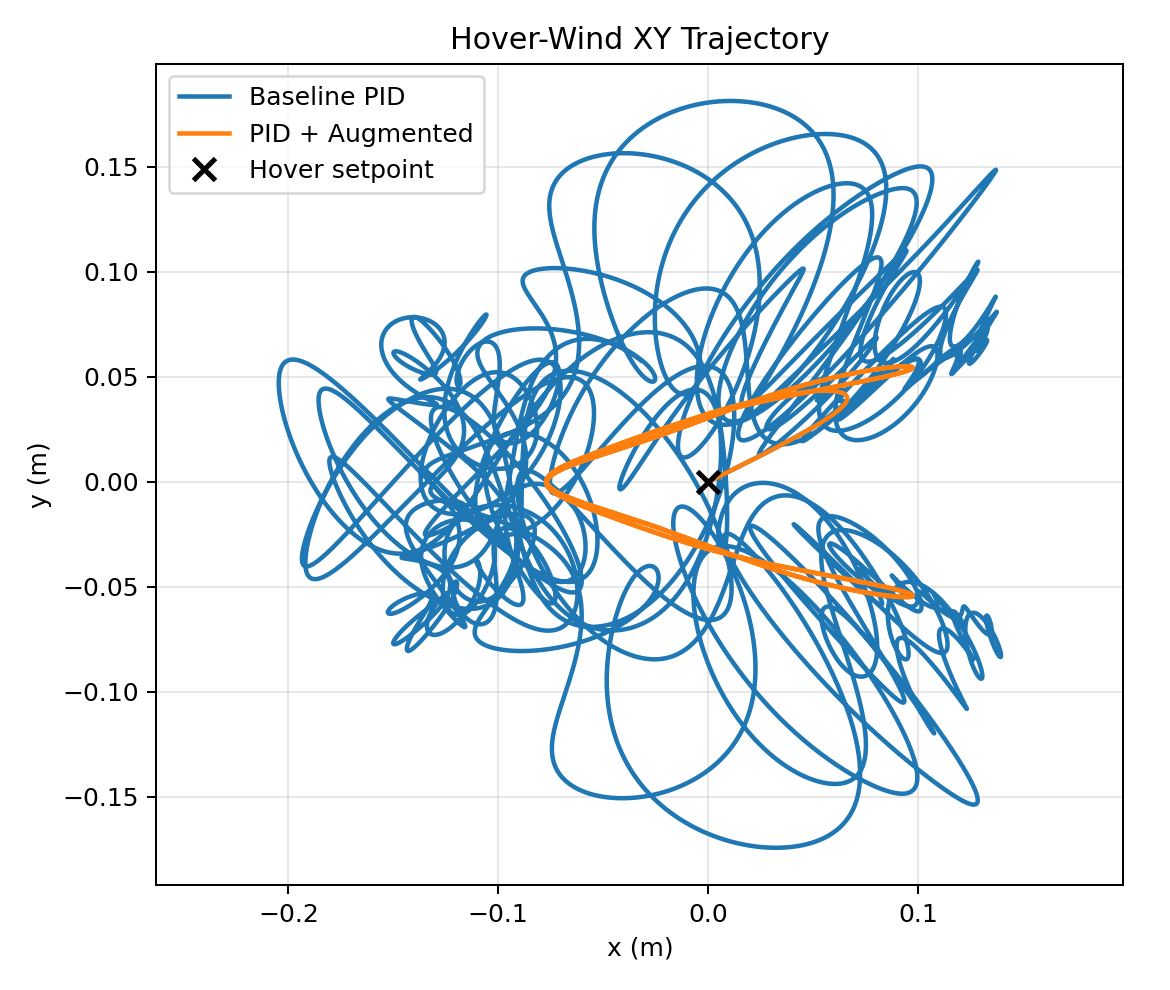
\includegraphics[width=0.72\linewidth]{fig_xy_trajectory.png}
\caption{XY hover trajectories under the same wind disturbance.}
\end{figure}

\begin{figure}[h!]
\centering
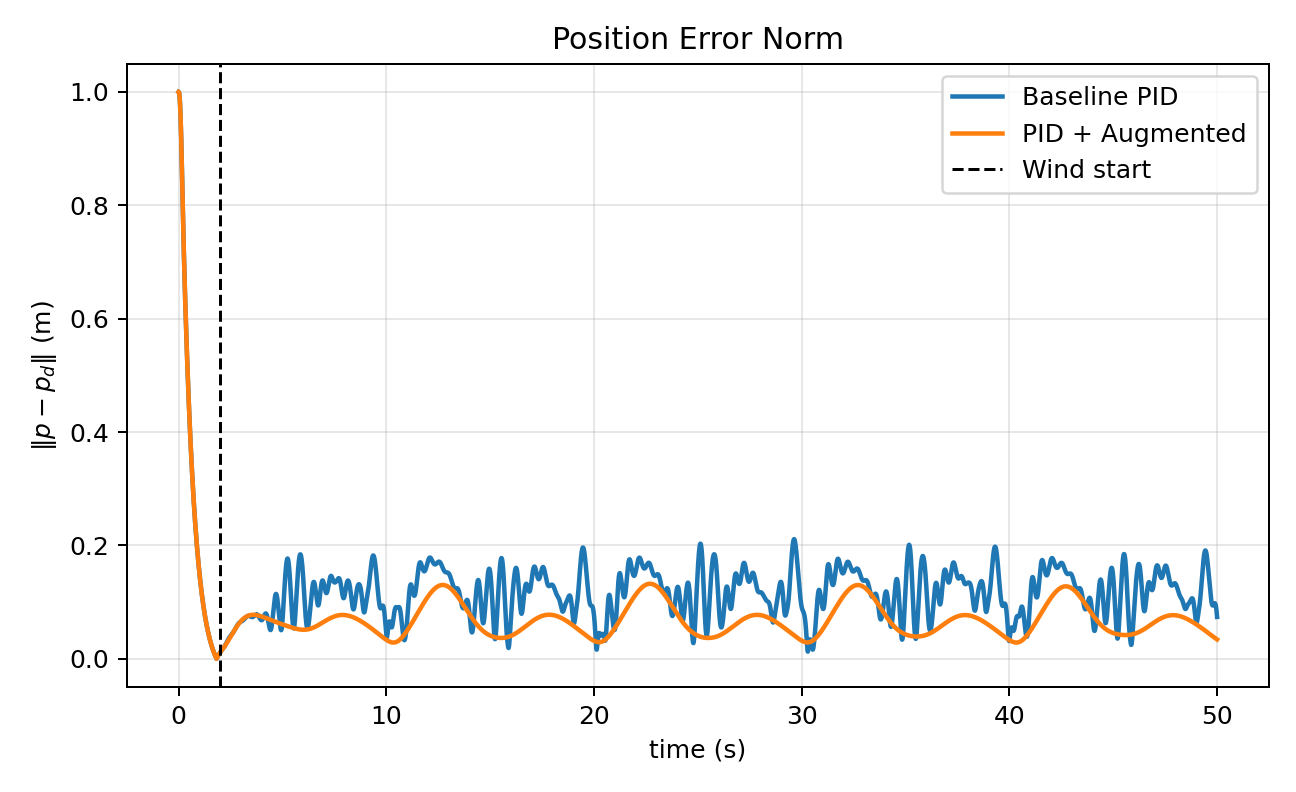
\includegraphics[width=0.78\linewidth]{fig_error_norm.png}
\caption{Position error norm over time. The dashed line marks wind start.}
\end{figure}

\begin{figure}[h!]
\centering
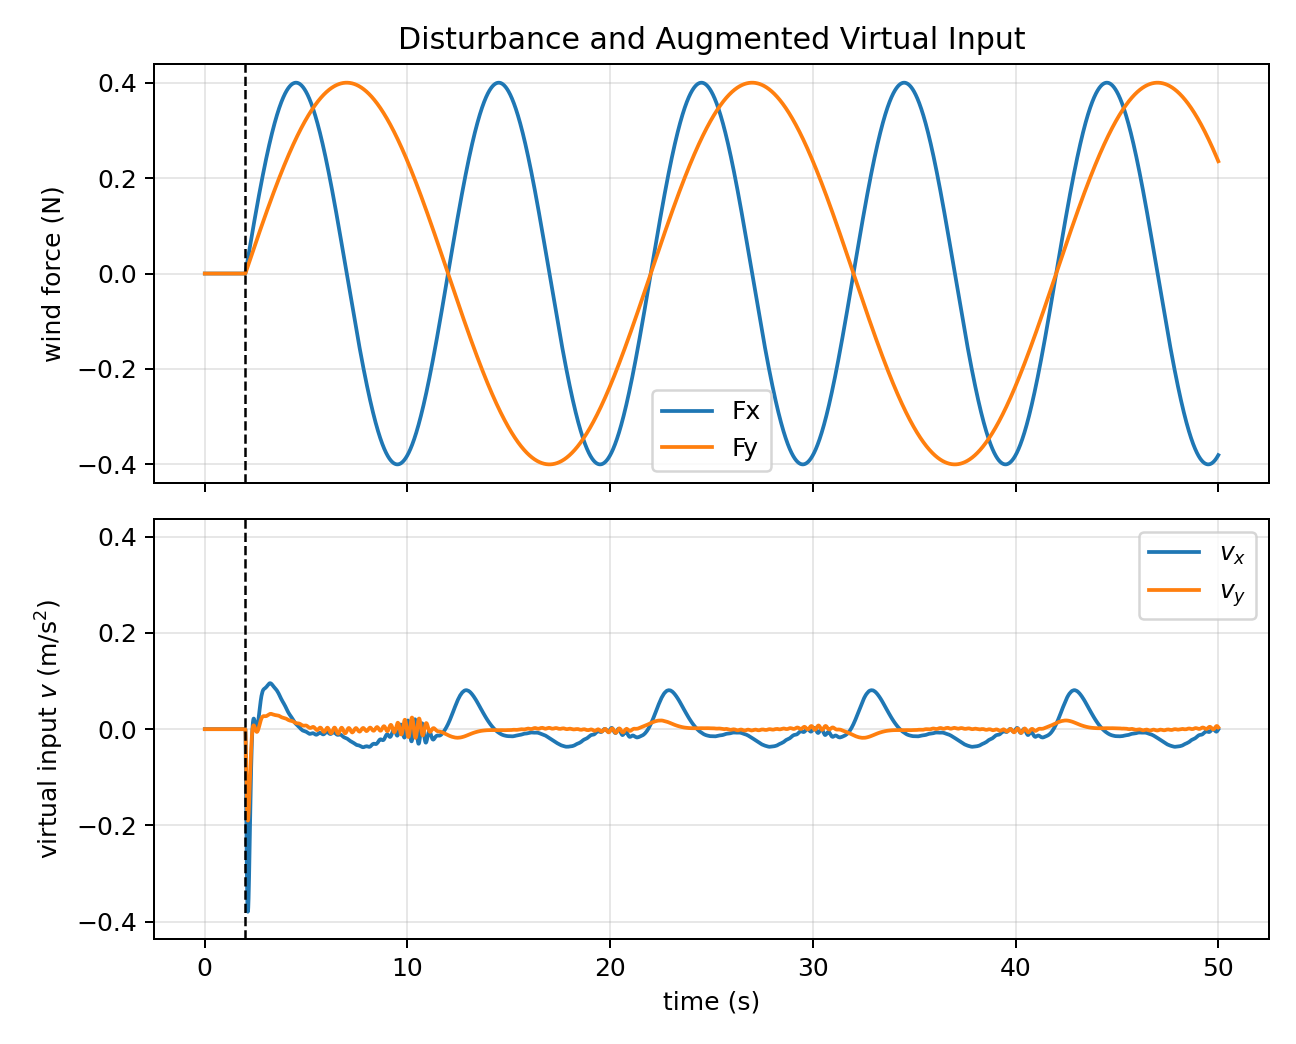
\includegraphics[width=0.78\linewidth]{fig_aug_signals.png}
\caption{Applied wind forces and augmented virtual inputs.}
\end{figure}

\begin{table}[h!]
\centering
\caption{Error Metrics (post-wind interval)}
\begin{tabular}{lccc}
\toprule
Metric & Baseline PID & PID + Augmented & Improvement (\%) \\
\midrule
Max position error [m] & 0.2111 & 0.1323 & 37.30 \\
RMS error [m] & 0.1223 & 0.0724 & 40.79 \\
\bottomrule
\end{tabular}
\end{table}

\section{Interpretation}
The augmentation does not replace the cascaded PID loops. It adds a bounded lateral correction term based on filtered model mismatch, then the baseline controller still performs acceleration-to-attitude and rate/moment control.

\end{document}
